%HW12.tex
%
% Twelfth Homework for Graduate Algebra
% Frank Sottile
%%%%%%%%%%%%%%%%%%%%%%%%%%%%%%%%%%%%%%%%%%%%%%%%%%%%%%%%%%%%%%%%%%%%%%%
\documentclass[12pt]{article}
\usepackage{multicol,amssymb,amsmath}
\usepackage{graphicx}
\usepackage{xcolor}
\headheight=8pt
%
\topmargin=-95pt
\textheight=744pt   \textwidth=575pt
\oddsidemargin=-60pt \evensidemargin=-60pt

\pagestyle{empty}

%%%%%%%%%%%%%%%%%%%%%%%%%%%%%%%%%%%%%%%%%%%%
\newcommand{\HH}{{\mathbb H}}
\newcommand{\FF}{{\mathbb F}}
\newcommand{\RR}{{\mathbb R}}
\newcommand{\CC}{{\mathbb C}}
\newcommand{\KK}{{\mathbb K}}
\newcommand{\NN}{{\mathbb N}}
\newcommand{\QQ}{{\mathbb Q}}
\newcommand{\TT}{{\mathbb T}}
\newcommand{\ZZ}{{\mathbb Z}}
\newcommand{\calA}{{\mathcal A}}
\newcommand{\calL}{{\mathcal L}}
\newcommand{\be}{{\bf e}}

\newcommand{\Hom}{\mbox{Hom}}
\newcommand{\End}{\mbox{End}}
\newcommand{\Mat}{\mbox{Mat}}
\newcommand{\rank}{\mbox{rank}}
\newcommand{\spec}{\mbox{spec}}
\newcommand{\cone}{\mbox{cone}}

\newcommand{\Square}{\raisebox{-2pt}{\includegraphics{figures/Square.eps}}}

\newcommand{\vect}[2]{(\begin{smallmatrix}#1\\#2\end{smallmatrix})}
\newcommand{\msp}{\hspace{8pt}}

\newcommand{\barsl}{\noindent\begin{minipage}[t]{575pt}
{\color{violet}\rule{575pt}{1.2pt}}\vspace{-5.7mm}\\
{\color{blue}\rule{575pt}{1.2pt}}\vspace{-5.7mm}\\
{\color{green}\rule{575pt}{1.2pt}}\vspace{-5.7mm}\\
{\color{yellow}\rule{575pt}{1.2pt}}\vspace{-5.7mm}\\
{\color{orange}\rule{575pt}{1.2pt}}\vspace{-5.7mm}\\
{\color{red}\rule{575pt}{1.2pt}}
\end{minipage}}


\def\demph#1{{\color{blue}{\sl #1}}}
\def\defcolor#1{{\color{blue}#1}}

\begin{document}
\LARGE 
\noindent
Algebra II\ \ Winter 2021 \hfill 12 April\makebox[40pt][l]{\ }\newline
Frank Sottile \hfill
\Large\sf
Twelfth Homework\makebox[40pt][l]{\ }
\vspace{5pt}
\normalsize

\noindent
Write your answers neatly, in complete sentences, and prove all assertions.
Start each problem on a new page (this makes it easier in Gradescope).
Revise your work before handing it in, and submit a .pdf  created from a LaTeX source to Gradescope.
Correct and crisp proofs are greatly appreciated; oftentimes your work can be shortened and made clearer.

\noindent
{\color{red}Due Monday 19 April.}\vspace{1pt}

\barsl

\begin{enumerate}
%%%%%%%%%%%%%%%%%%%%%%%%%%%%%%%%%%%%%
%\setcounter{enumi}{52}


%\newpage
%%%%%%%%%%%%%%%%%%%%%%%%%%%%%%%%%%%%%%%%%%%%%%%%%%%%%%%%%%%%%%%%%%%%%%%%%%%%%%%%%
\item {[15]}
  Let $f:=x^4+ax^2+b\in K[x]$ be an irreducible quartic over a field $K$ of characteristic not 2.
  Let $G$ be the Galois group of $f$.
  (Note that $f$ is separable, due to the characteristic being not 2.)
  Show that
  \begin{enumerate}
    \item If $b$ is a square in $K$, then $G=V$, the Klein four group.
    \item If $b$ is not a square in $K$, but $b(a^2-4b)$ is a square, then $G\simeq \ZZ/4\ZZ$ is a cyclic group.
    \item If neither $b$ nor $b(a^2-4b)$ are squares in $K$, then $G\simeq D_4$, the dihedral group.
  \end{enumerate}
\vspace{-2pt}
%%%%%%%%%%%%%%%%%%%%%%%%%%%%%%%%%%%%%%%%%%%%%%%%%%%%%%%%%%%%%%%%%%%%%%%%%%%%%%%%%

%\newpage
%%%%%%%%%%%%%%%%%%%%%%%%%%%%%%%%%%%%%%%%%%%%%%%%%%%%%%%%%%%%%%%%%%%%%%%%%%%%%%%%%
\item {[20]} Determine the Galois groups of the following polynomials over $\QQ$. 
  \begin{enumerate}
    \item $x^4+4x+4$
    \item $x^4+3x+3$
    \item $x^4-7x^2-3x+1$
    \item $x^5-3x+1$
  \end{enumerate}
\vspace{-2pt}
%%%%%%%%%%%%%%%%%%%%%%%%%%%%%%%%%%%%%%%%%%%%%%%%%%%%%%%%%%%%%%%%%%%%%%%%%%%%%%%%%

%\newpage
%%%%%%%%%%%%%%%%%%%%%%%%%%%%%%%%%%%%%%%%%%%%%%%%%%%%%%%%%%%%%%%%%%%%%%%%%%%%%%%%%
\item   Suppose that $F/K$ is a Galois extension of degree $p^n$ for $p$ a prime and $n$ a positive integer.
        Prove that for every degree $d$ dividing $p^n$, (e.g. $d\in\{1,p,p^2,\dotsc,p^n\}$) $F/K$ has an intermediate field $E$ with the
        degree of $E/K$ equal to $d$ and $E/K$ is Galois.
   \vspace{-2pt}
%%%%%%%%%%%%%%%%%%%%%%%%%%%%%%%%%%%%%%%%%%%%%%%%%%%%%%%%%%%%%%%%%%%%%%%%%%%%%%%%%

%\newpage
%%%%%%%%%%%%%%%%%%%%%%%%%%%%%%%%%%%%%%%%%%%%%%%%%%%%%%%%%%%%%%%%%%%%%%%%%%%%%%%%%
\item Show that  $\QQ(\sqrt{2+\sqrt{2}})$ is a Galois extension of $\QQ$, determine its Galois group, and determine all intermediate fields.
   \vspace{-2pt}
%%%%%%%%%%%%%%%%%%%%%%%%%%%%%%%%%%%%%%%%%%%%%%%%%%%%%%%%%%%%%%%%%%%%%%%%%%%%%%%%%


\end{enumerate}
%%%%%%%%%%%%%%%%%%%%%%%%%%%%%%%%%%%%%%%%%%%%%%%%%%%%%%%%%%%%%%%


{\color{red}Corrections: }

In  the first problem, suppose that a polynomial $f\in K[x]$ splits into linear factors in some extension field $F$ of $K$.
Then $f$ has a multiple root in $F$ if and only if $f$ and its formal derivative $f'$ have a common factor (this is done in Chapter III).
But then they have a common factor in $K[x]$.
Consequently, if $f$ is irreducible in $K[x]$, it is not separable if and only if $f'=0$.
But then (necessarily) the characteristic of $K$, $p$, divides the degree of $f$, and a little more thought leads to the conclusion that
there is a polynomial $g\in K[x]$ with $f(x)=g(x^p)$.

The reason for this discourse is to see that in the first problem, forbidding $K$ to have characteristic 2, a polynomial of the given form
is irreducible is then necessarily separable.\bigskip

2(b)  had a typo, the quintic is $x^5-3x+1$, and not $x^5-2x+1=(x-1)(x^4+x^3+x^2+x-1)$.



\end{document}
